\documentclass[12pt,oneside,					% 1 bzw. 2-seitiger Druck				
parskip=half, 				% definiert Absätze (false[default]/half/full oder true/false)
captions=tableabove, 		% Tabellenüberschriften
captions=figurebelow, 		% Bildunterschriften
open=any,                   % Neue Kapitel drüfen rechts und links beginnen
titlepage=firstiscover,     % Titelseite auf 1. Seite
final  %final/ draft		% draft/final entscheidet z.B. ob Bilder drin sind oder nur sw-dummy
]{scrbook} % scrbook aus KOMA, empfohlen, da europäisch angepasst (oder scrartcl)


%%% Eingabe weiterer Pakete zur Anpassung
\usepackage{setspace}		% Zeilenabstände
\onehalfspacing				% nicht direkt 1,5-facher WORD-Abstand!
\usepackage[english, ngerman]{babel} 						% neue Rechtschreibung durch n(ew)german (auch Silbentrennung), letzte Sprache ist Hauptsprache
\usepackage[utf8]{inputenc}  								% inputencoding [eingabecodierung, enthält z.B. ß,ö,ä,...]
\usepackage[T1]{fontenc} 									% fontencoding (Zeichensatz, Ausgabe)
\usepackage[autostyle=true,german=guillemets]{csquotes} 	% korrekte Zitierart in allen babel-Sprachen --> \enquote; ohne guillemets: Hochkommata
\usepackage[newcommands] {ragged2e} 						% Silbentrennung, bei rechts-/ linksbündig
\usepackage{array} 											% für Tabellen und auch Mathe möglich; empfohlen: immer verwenden!
\usepackage{booktabs} 										% für Striche  in Tabellen in 3 versch. Dicken
\usepackage{graphicx}										% für Bilder (jpg,png,pdf)
\graphicspath{{../Bilder/}}
\usepackage{xcolor} 										% für Farben (rgb,  RGB, CMYK, cmyk, named, HTML,...) ; kleine Buchstaben: [%], große: [8Bit, also 0...255]
\usepackage{wrapfig} 										% von text umflossene Bilder
\usepackage[style=numeric]{biblatex} 						% Quellenverweise
\usepackage[intoc,german]{nomencl} 							% Nomenklatur, Fremdwortverzeichnis --> vor dem Text!
\makenomenclature
\usepackage[locale = DE, per-mode = symbol]{siunitx} 					% für die einfachere Eingabe von Einheiten: \SI{30}{\meter}; Es gibt Einstellmöglichkeiten --> Dokumentation (cmd, dann texdoc NamedesPakets)
\usepackage{amsmath} 										% komplexere Mathe möglich
\renewcommand{\theequation}{\arabic{equation}}				% Gleichungsnummern kapitelunabhängig durch modifikation d. Counters
\usepackage{enumitem}										% Anpassbare Aufzählung mit enumerate
\usepackage{lmodern}										% druckt "normal" dicken Text
%\newcommand{\RN}[1]{\uppercase\expandafter{\romannumeral#1}} % große röm. Zahlen
\usepackage{xspace} % für C++
\usepackage{amsmath} % schöne Matrixdarstellung
\usepackage{tabularx}
\usepackage{listings}
\usepackage{float}

% Define colors for code highlighting
\definecolor{keyword}{RGB}{0,0,255} % Blue for keywords
\definecolor{comment}{RGB}{0,128,0} % Green for comments
\definecolor{string}{RGB}{163,21,21} % Red for strings
\definecolor{background}{RGB}{240,240,240} % Light gray background
\definecolor{lightgray}{rgb}{.9,.9,.9}
\definecolor{darkgray}{rgb}{.4,.4,.4}
\definecolor{purple}{rgb}{0.65, 0.12, 0.82}
\definecolor{blue}{rgb}{0.1, 0.1, 0.9}
\definecolor{red}{rgb}{0.8, 0.1, 0.1}


% Global style (base style for all listings)
\lstdefinestyle{globalstyle}{
    backgroundcolor=\color{lightgray}, % Light gray background
    basicstyle=\ttfamily\footnotesize, % Monospace font, smaller size
    frame=single,                      % Add a frame around the content
    breaklines=true,                   % Wrap long lines
    captionpos=b,                      % Caption at the bottom
    numbers=left,                      % Line numbers on the left
    numberstyle=\tiny\color{darkgray}, % Small font for line numbers
    showspaces=false,                  % Don't show spaces
    showstringspaces=false,            % Don't show spaces in strings
    tabsize=4                          % Tab size
}
\lstset{style=globalstyle} % Set global style

% Python-specific style
\lstdefinestyle{pythonstyle}{
    keywordstyle=\color{blue}\bfseries, % Blue, bold keywords
    stringstyle=\color{red},           % Red for strings
    commentstyle=\color{green}\itshape, % Green, italic comments
}

% TypeScript-specific style
\lstdefinestyle{typescriptstyle}{
    keywordstyle=\color{purple}\bfseries, % Purple, bold keywords
    stringstyle=\color{orange},           % Orange for strings
    commentstyle=\color{gray}\itshape,    % Gray, italic comments
}

% Logfile-specific style
\lstdefinestyle{logfilestyle}{
    basicstyle=\ttfamily\small,          % Monospace font, slightly larger size
    backgroundcolor=\color{white},       % White background
    commentstyle=\color{red},            % Red for comments (e.g., ERROR)
    keywordstyle=\color{black},          % Black for general text
    frame=none,                          % No frame for log files
    numbers=none                         % No line numbers
}

% Python language definition
\lstdefinelanguage{Python}{
    keywords={def, return, if, else, for, while, import, from, as, class, self, lambda, try, except},
    ndkeywords={True, False, None},
    sensitive=true,
    comment=[l]{\#},
    stringstyle=\color{red}\ttfamily,
    morestring=[b]',
    morestring=[b]",
}

% TypeScript language definition
\lstdefinelanguage{TypeScript}{
    keywords={interface, export, string, number, boolean, let, const, async, await, function, return, if, else, for, while, switch, case, break},
    ndkeywords={class, readonly, implements, extends, private, public, protected, static, declare, type, enum, namespace, module, from, as},
    sensitive=true,
    comment=[l]{//},
    morecomment=[s]{/*}{*/},
    stringstyle=\color{orange}\ttfamily,
    morestring=[b]',
    morestring=[b]",
    morestring=[b]`
}

\usepackage[pdfpagelayout=TwoPageLeft]{hyperref} 										% klickbare Links/URLs --> sollte letztes Paket sein!! href ermöglicht externe Adressen zu verlinken; \hypersetup{keyvals} ermöglich Optionen 
\usepackage[all]{hypcap} 									% sorgt für 


%% Neuen Spaltentyp definieren
\newcolumntype{H}{%
	>{\footnotesize} c} % Header

%% Definition der Daten für die Titelseite
\author{Yan Ohainski} 
\title{Entwicklung eine KI-basierten Meetingassistenten zur Darstellung und Aufbereitung gesprochener Inhalte}
%\subtitle{Simulation in MATLAB Simulink} 
\date{\today}
%\titlehead{Titelkopf}
\subject{%\newpage
	Masterarbeit}

\publishers{
	\vspace{1.0cm}
	an der Hochschule für angewandte Wissenschaft und Kunst
 
    Prüfer:
    
    Prof. Dr. rer. nat. Roman Grothausmann
    
    Betreuer:
    
	Henri Reumschüssel
	
	\vspace{3cm}
	\centering
	
\includegraphics[height=3.cm]{Bilder/hawk-fi-logo.pdf}\\
}	



%Literaturdatenbank verlinken
%\addbibresource{lib_masterarbeit.bib}

%Fremdwortverzeichnis 
\PassOptionsToPackage{intoc,nomentbl}{nomencl}
\renewcommand{\nomname}{Fremdwortverzeichnis}
\newcommand{\fremdwort}[2]{#1\nomenclature{\textbf{#1}}{#2}}



%Gleichungsnummerierung
\numberwithin{equation}{chapter} %sets equation numbers



\begin{document} 
\setcounter{tocdepth}{1} % Tiefe des Inhaltsverzeichnis einstellen: nur caption und section
\maketitle				% Titelseite einfügen
%\input{Deckblatt}
%\thispagestyle{empty}
%\mbox{}

\frontmatter			% erste Seiten römisch nummerieren

% Inhalts-, Tabellen-, Bild-, Fremdwortverzeichnis
\tableofcontents

\listoftables
\addcontentsline{toc}{chapter}{Tabellenverzeichnis}
\listoffigures
\addcontentsline{toc}{chapter}{Abbildungsverzeichnis}
% \printnomenclature
%\addcontentsline{toc}{chapter}{Eigenständigkeitserklärung \& Nutzungsrecht}	 	
\chapter{Eigenständigkeitserklärung \& Nutzungsrecht}
\subsubsection{Erklärung bzgl. des Einsatz von IT-/KI- gestützten Schreibwerkzeugen:}

\textbf{Erklärung}

Hiermit versichere ich, dass die vorliegende Arbeit mit dem Titel \textit{Entwicklung eines KI-basierten Meetingassistenten zur Darstellung und Aufbereitung gesprochener Inhalte} selbständig von mir und ohne fremde Hilfe verfasst worden ist, dass keine anderen Quellen und Hilfsmittel als die angegebenen benutzt worden sind und dass die Stellen der Arbeit, die anderen Werken - auch elektronischen Medien - dem Wortlaut oder Sinn nach entnommen wurden, durchgängig unter Angabe der Quelle kenntlich gemacht worden sind. Dies gilt auch für Zeichnungen, Skizzen, bildliche Darstellungen und dergleichen.

Ich erkläre hiermit, dass ich beim Einsatz von IT-/KI-gestützten Schreibwerkzeugen diese Werkzeuge unter der Rubrik \textit{Übersicht verwendeter Hilfsmittel} (\ref{sec:hilfsmittel}) mit ihrem Produktnamen, meiner Bezugsquelle und einer Übersicht des im Rahmen dieser Arbeit genutzten Funktionsumfangs vollständig aufgeführt habe. Die mit IT-/KI-gestützten Schreibwerkzeugen erstellten Inhalte habe ich steuernd bearbeitet.

Ich versichere, dass ich die vorliegende Arbeit oder Teile daraus nicht anderweitig als Prüfungsarbeit eingereicht habe oder diese als Veröffentlichung erschienen ist.

\vspace{1cm}

\noindent
\begin{minipage}[t]{0.45\textwidth}
    \rule{5cm}{0.4pt} \\ 
    \textbf{Ort, Datum}
\end{minipage}%
\hfill
\begin{minipage}[t]{0.45\textwidth}
    \rule{5cm}{0.4pt} \\ 
    \textbf{Unterschrift}
\end{minipage}

\subsubsection{Erklärung zu Nutzungsrechten und Verwertungsrechten}
Ich bin hiermit einverstanden, dass von meiner Abschlussarbeit (ggf. nach Ablauf der Sperre) ein
Vervielfältigungsstück erstellt werden kann, um es der Bibliothek der HAWK zur Verfügung zu
stellen und Dritten öffentlich zugänglich zu machen.
Ich erkläre, dass Rechte Dritter der Veröffentlichung nicht entgegenstehen.

\vspace{1cm}

\noindent
\begin{minipage}[t]{0.45\textwidth}
    \rule{5cm}{0.4pt} \\ 
    \textbf{Ort, Datum}
\end{minipage}%
\hfill
\begin{minipage}[t]{0.45\textwidth}
    \rule{5cm}{0.4pt} \\ 
    \textbf{Unterschrift}
\end{minipage}


\vspace{1cm}
\subsubsection{Sperrvermerk der Abschlussarbeit}

\noindent 
\vspace{5mm}

\noindent
\fbox{\rule{0pt}{1em}\hspace{1em}} \textbf{Kein Sperrvermerk} \\
\noindent
\fbox{\rule{0pt}{1em}\hspace{1em}} \textbf{Sperrvermerk}

\vspace{1cm}

\noindent
\begin{minipage}[t]{0.45\textwidth}
    \rule{5cm}{0.4pt} \\ 
    \textbf{Ort, Datum}
\end{minipage}%
\hfill
\begin{minipage}[t]{0.45\textwidth}
    \rule{5cm}{0.4pt} \\ 
    \textbf{Unterschrift}
\end{minipage}

\mainmatter				% Ab hier arabische Nummerierung

%% Die einzelnen Teile einfügen
\chapter{Einleitung}
Die fortschreitende Digitalisierung und die zunehmende globale Vernetzung von Unternehmen führen zu einer stetig wachsenden Bedeutung effizienter Kommunikations- und Informationsprozesse. Insbesondere im modernen Büroumfeld stellen Meetings ein zentrales Element der Zusammenarbeit dar. Sie dienen der Abstimmung, Entscheidungsfindung und Koordination von Arbeitsabläufen. Gleichzeitig steigt jedoch mit der Anzahl und Dauer von Besprechungen auch der organisatorische Aufwand, der mit deren Vor- und Nachbereitung verbunden ist.

Trotz der Verbreitung moderner Kommunikationsplattformen wie Chat-Systemen oder Videokonferenzlösungen bleibt die strukturierte Dokumentation von Meetings eine Herausforderung. Häufig fehlen Zeit und Ressourcen, um besprochene Inhalte vollständig und nachvollziehbar festzuhalten. In der Praxis führt dies oftmals dazu, dass Informationen verloren gehen, Entscheidungen nicht eindeutig dokumentiert werden oder Themen mehrfach diskutiert werden müssen. Insbesondere in Arbeitsumgebungen mit hoher Taktung an Meetings entsteht dadurch eine erhebliche Informationsdichte, die von den Beteiligten kaum effizient verarbeitet werden kann.

Ein möglicher Ansatz zur Bewältigung dieser Problematik liegt im Einsatz KI-gestützter Systeme zur automatisierten Verarbeitung gesprochener Sprache. Moderne Verfahren der automatischen Spracherkennung und Textverarbeitung ermöglichen es, gesprochene Inhalte in Textform zu überführen, zu strukturieren und zusammenzufassen. In der Praxis zeigen sich jedoch weiterhin Herausforderungen hinsichtlich Genauigkeit, zeitlicher Verfügbarkeit der Ergebnisse sowie der sinnvollen Aufbereitung der Informationen. Insbesondere nachträglich erzeugte Zusammenfassungen sind fehleranfällig oder stehen nicht unmittelbar zur Verfügung, wodurch ihr Nutzen im Arbeitsalltag eingeschränkt wird.

Vor diesem Hintergrund befasst sich diese Masterarbeit mit der Entwicklung eines KI-basierten Meetingassistenten zur automatisierten Erfassung, Aufbereitung und Darstellung gesprochener Inhalte. Ziel ist es, ein System zu konzipieren und umzusetzen, das Meetings in Echtzeit analysiert, relevante Inhalte strukturiert aufbereitet und dadurch die Nachbereitung von Besprechungen deutlich erleichtert. Der Fokus liegt dabei auf der praktischen Umsetzbarkeit sowie der Integration moderner Verfahren aus den Bereichen Sprachverarbeitung und Automatisierungstechnik.

Die Arbeit ist im Studiengang Elektro- und Informationstechnik mit der Vertiefung Automatisierung und Robotik angesiedelt und verbindet theoretische Konzepte der künstlichen Intelligenz mit einer anwendungsnahen technischen Umsetzung. Ziel ist es, einen Beitrag zur Effizienzsteigerung wissensbasierter Arbeitsprozesse zu leisten und das Potenzial KI-gestützter Assistenzsysteme im beruflichen Kontext aufzuzeigen.

\section{Notisent}
Notisent GmbH ist ein 2025 gegründetes Technologie-Start-up mit Sitz in Göttingen, das sich auf die Entwicklung KI-gestützte Arbeitsassistenten für wissensintensive Arbeitsprozesse spezialisiert hat. 
Ziel des Unternehmens ist es, die zunehmende Informationsdichte in digitalen Arbeitsumgebungen durch automatisierte Analyse- und Strukturierungsmechanismen beherrschbar zu machen und dadurch die Effizienz sowie die Qualität wissensbasierter Tätigkeiten zu erhöhen. 
Das Unternehmen entwickelt einen intelligenten digitalen Assistenten, der es Mitarbeitenden und Organisationen ermöglicht, den täglichen Informations- und Kommunikationsfluss effizienter zu bewältigen. Im Zentrum der Lösung steht eine KI-Plattform, die E-Mail, Dokumente, Notizen, Kalenderinformationen und andere Datenquellen analysiert, verknüpft und priorisiert, um arbeitsrelevante Inhalte und Aufgaben gezielt bereitzustellen. 

\section{Gegenstand und Ziel}
Ziel der Arbeit ist die Entwicklung eines Meetingassistenten-Prototypen, welcher in Echtzeit in der Lage ist gesprochene Inhalte in einem Online-Meeting zu analysieren und anschließend mithilfe von KI für den Benutzer grafisch aufzubereiten. Dazu sollen im ersten Kapitel die notwendigen Grundlagen geschaffen werden für Technisches Verständnis. Im zweiten Kapitel Methodik soll dem Leser die herangehensweise an das Projekt vermittelt werden und anschließend im darauffolgenden Kapitel die Umsetzung des Prototypen. 

Der Meetingassistent wird im Webframework Django in der Programmiersprache Python entwickelt. Die Grundlage des Meetingassistenten bildet ein Large Language Modell, welches auf Servern des KI-Servicezentrums für sensible und kritische Infrastruktur in Göttingen gehostet wird. 

Insgesamt liegt der Fokus auf der Entwicklung eines ersten funktionsfähigen Prototypen, welcher in die Notisent Umgebung eingebunden werden kann. In Abbildung X ist eine Übersicht über alle Komponenten dargestellt. 

Grafik wie grundsätzlich funktionieren soll 

Anhand der folgenden Forschungsfragen wird präzisiert, welche Ergebnisse diese Arbeit leifert. 
Forschungsfragen:
\begin{enumerate}
    \item\textbf{Wie kann ein Live-Meetingassistent entwickelt werden?} 

Diese Frage untersucht wie so ein Live-Meetingassistent vom Grundkonzept her aufgebaut werden muss um funktioniern zu können. 

    \item\textbf{Was für Anforderungen muss so ein Meetingassistent erfüllen?}

In diesem Zusammenhang soll untersucht werden, welche Anforderungen ein Meetingassistent erfüllen muss um einen Mehrwert für ein Meeting zu bieten. 

    \item\textbf{Wie ist die Qualität im vergleich zu Komplett zusammengefassten Meetings?} 

Es wird erforscht, wie sich ein Live-Meetingassistent im vergleich zu bereits bestehenden Tools zum zusammenfassen 

    \item\textbf{Kann die Zusammenfassung in annehmbarer Zeit erstellt werden?} 
    
\end{enumerate}

Diese Forschungsfragen bilden die Grundlage für die Entwicklung eines leistungsfähigen, flexiblen und nutzerfreundlichen KI-Meetingassistenten, welcher sich in die Notisent Umgebung integrieren lässt und 
 

 
 



\chapter{Grundlagen}
In diesem Kapitel werden alle notwendigen Hintergrundinfos zum Verständnis der Arbeit gegeben.

\section{Transformer}
Die Architektur des Transformer Modells wurde erstmals 2017 von Vaswani \textcite{Vaswani2017} vorgestellt und stellt eine fundamentale Neuerung im Bereich der neuronalen Netze und natürlicher Sprachverarbeitung dar (NLP) dar. Die Transformer-Architektur verzichtet vollständig auf rekurrente oder konvolutionale Mechanismen und setzt stattdessen auf einen Selbstaufmerksamkeitmechanismus(Self Attention). Dadurch übertreffen Transformermodelle ältere Modelle wie rekurrente neuronale Netze (RNNs) und Convolutional Neural Networks )CNN) in vielen Anwendungsfällen wie Kontextverständniss, Parallelisierbarkeit und Skalierbarkeit. Darüber hinaus können Transformermodelle universell in verschiedenen Bereichen eingesetzt werden. Die Transformer Architektur bildet die Grundlage für nahezu alle aktuell großen Sprachmodelle wie z.B. BERT, GPT oder T5

In der folgenden Abbildung ist der orignale Aufbau eines Transformermodells schematisch dargestellt

\begin{figure}
\centering
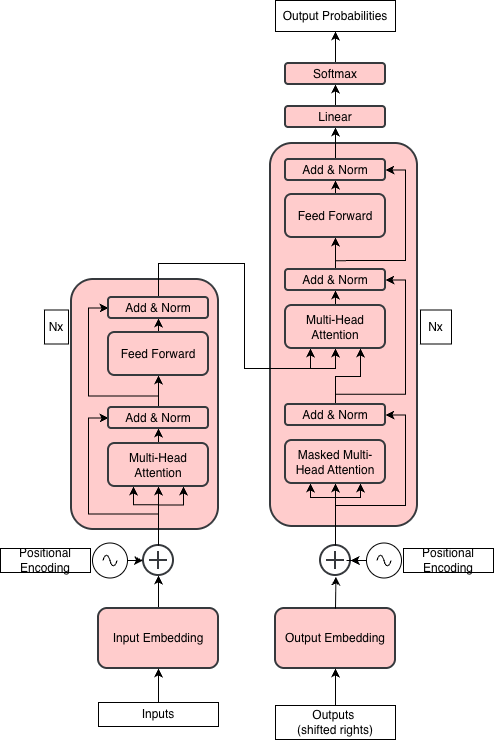
\includegraphics[height=0.7\textheight]{Bilder/encoder_decoder_transformer.drawio.png}
\caption{Decoder-Only Transformer in Anlehnung an  und }
\label{fig:decoder}
\end{figure}

In der originalen, von Vaswani u.a. vorgestellte Transformer Architektur besteht aus Encoder- und Decoderschichten. Der Encoder ist verantwortlich für die Verarbeitung des Eingabetexts und erzeugt daraus eine Reihe kontextualisierter Repräsentationen, welche vom Decoder genutzt werden um Ausgaben, wie einen übersetzten oder vorhergesagten Text, zu generieren. 

Encoder- und Decoderschichten können unabhängig voneinander für Modelle genutzt werden, so hat sich die ursprüngliche Architektur zu drei Architekturrichtungen weiterentwickelt. Encoder-Only (BERT), Decoder-Only(GPT-Modelle) und Encoder-Decoder (T5) eigenen sich für verschiedene Anwendungsgebiete.

Jeder Encoder und Decoder besteht aus weiteren Schichten

Ein zentraler Bestandteil der Transformerarchitektur ist der Selbstaufmerksamkeitsmechanismus (Self-Attention), welcher es ermöglicht kontextuelle Zusammenhänge zwischen den Tokens zu erkennen. Bei diesem werden allen Tokens in der Eingabesequenz Werte je nach relevanz für den Gesamtkontext zugewiesen, wodurch Zusammenhänge über große Distanzen nicht verloren gehen. Die parallele Verarbeitung steigert die Effizienz sowie Qualität der Ausgabe immens, da Tokens nicht sequientiell nacheinander abgearbeitet werden wie bei RNN oder LSTM Modellen.

\begin{itemize}
    \item Self-Attention-Schicht:  
    \item Feed-Forward-Schicht
    \item Residualverbindung und Normalisierung
    
\end{itemize}

1. Self-Attention-Schicht: Berechnung der Beziehung zwischen allen Positionen einer Sequenz
2. Feed-Forward-Schicht: Vearbeitung gewonnener Information
3. Residualverbindung und Normalisierung: Stabilisierung des Trainings und verbessern des Informationsflusses zwischen schichten. 



Besonders GPT 
Generative Pretrained Transformer
Bild mit Aufbau vom Transformer Original und daran beschreiben wie aufgebaut ist 

Vortraining und Finetuning

Anwendungsbereiche für Transformer und bekannte Modelle mit Transformer Architektur
Nachteile im Vergleich zu anderen KI-Modellen 
Darüber hinaus lassen sich Transformer auch für andere Zwecke einsetzten als zur NLP. Transformer werden allerdings nicht ausschließlich für NLP verwendet und finden auch Anwendung in bereichen wie Bildverarbeitung und Audioverarbeitung
-> Whisper als Text to Speech Transformer modell 


\section{Speech-to-Text}
Speech to text bezeichnet die technik um aus gesprochenem inhalt 
Was ist das? Wie funktiniert das? Welche Technik wird hier verwendet? 
Verweis auf Masterprojekt. Wie wurde ausgewähltes Modell feingetuned, bzw wie wird es finegetuned. 
Whisper funktioniert wie ein Transformer, bei dem anstatt wörtern log mel spektogramme ein
Kann ins Detail gehen
Kurz anreißen wie sich technik entwickelt hat, ohne zu sehr ins Detail zu gehen, keine größere Relevanz
Faster Whisper, welches auf Whisper basiert (lediglich inferenz ist anderes) 

Speech-to-Text (STT) auch Automatic Speech Recognition (ASR) beschreibt alle rechnergestützten Verfahren zur automatisierten Umwandlung gesprochener Sprache in schriftliche Form. Ziel ist die robuste Erkennung von Sprache, deren korrekter Interpretation sowie Generierung einer konkreten Textrepräsentation. 

Das Modell Whisper wurde 2022 von OpenAI veröffetnlicht und ist im wesentlichen ein Encoder-Decoder-Transformermodell, welches mit annotierten Audiodaten Trainiert wurde. Dabei verarbeitet der Encoder anstatt Text, Mel-Sektrogramme des Audios mit welchem der Decoder anschließend Text-Tokens verarbeitet. 

Whisper wurde mit etwa 680.000 Stunden multilingualem Audiomaterial trainiert, was es zu einem guten Foundation Modell im Bereich der ASR macht. Durch Finetuning von Whisper lässt sich das Modell darüber hinaus weiter an eigene Bedürfnisse anpassen. 


Encoder: Wandelt das Audiosignal (Mel-Spektogramm) in eine latente Repräsentation um. 

Decoder: Erzeugt auf Basis dieser Repräsentation Text-Token ähnlich wie ein Sprachmodell. 

\section{Large-Language-Model}
Large Language Models (LLMs) sind tiefenlernende neuronale Netze, die auf umfangreichen Sammlungen natürlicher Sprachdaten trainiert werden, um sowohl sprachliches Verständnis als auch generative Fähigkeiten zu entwickeln. Im Gegensatz zu älteren, stärker auf spezifische Aufgaben zugeschnittenen NLP-Modellen entstehen durch das Training auf breit gefächerten Textkorpora allgemeine, domänenübergreifende Sprachfertigkeiten. Daher werden moderne LLMs häufig als Foundation Models bezeichnet, da sie eine vielseitige Grundlage für eine Vielzahl nachgelagerter Anwendungen bieten (Zhao et al., 2023; Minaee et al., 2024).

Technologisch basieren die meisten heutigen LLMs auf der Transformer-Architektur, die durch Mechanismen wie Self-Attention eine effiziente Verarbeitung langer Textsequenzen ermöglicht und damit die zuvor gängigen rekurrenten Modelle weitgehend abgelöst hat. Ein charakteristisches Merkmal von LLMs ist ihre enorme Größe: Sie umfassen häufig Milliarden von Parametern und werden auf Datensätzen im Größenbereich vieler hundert Gigabyte bis hin zu mehreren Terabyte trainiert. Empirische Scaling Laws zeigen, dass mit wachsenden Modellparametern, größeren Datensätzen und höherer Rechenleistung systematisch Leistungssteigerungen erzielt werden können (Zhao et al., 2023).

Der Trainingsprozess moderner LLMs erfolgt in zwei Schritten. Zunächst werden die Modelle im Pre-Training mittels selbstüberwachtem Lernen trainiert. Typische Lernziele sind das Vorhersagen des nächsten Tokens oder das Auffüllen maskierter Textteile. Dieser Prozess führt zu einer breit angelegten, generalistischen Sprachkompetenz. Darauf aufbauend folgt das Fine-Tuning, bei dem ein vortrainiertes Modell durch überwachtes Lernen auf spezifische Aufgaben oder Daten angepasst wird. Fine-Tuning kann das gesamte neuronale Netz betreffen, jedoch haben sich in den letzten Jahren auch parameter-effiziente Methoden wie LoRA (Low-Rank Adaptation) etabliert. Bei LoRA werden nur kleine, trainierbare Zusatzmatrizen ergänzt, während der Großteil der ursprünglichen Modellparameter eingefroren bleibt. Dies reduziert den Rechenaufwand erheblich und ermöglicht die Anpassung großer Modelle auf vergleichsweise kleinen Datensätzen.

Ein weiteres Schlüsselmerkmal aktueller LLMs ist ihre Fähigkeit zu In-Context Learning. Das Modell nutzt dabei allein auf Basis der im Prompt bereitgestellten Beispiele oder Instruktionen neue Aufgabenstrukturen, ohne dass Parameteränderungen notwendig sind. Damit entsteht eine bemerkenswerte Flexibilität: Das Modell kann Aufgaben lösen, für die es nie explizit trainiert wurde, sofern die Aufgabenbeschreibung im Kontext ausreichend präzise ist.

Die Entwicklung von LLMs markiert einen Paradigmenwechsel in der Sprachverarbeitung. Während klassische Sprachmodelle primär die Wahrscheinlichkeit des nächsten Tokens schätzten, generieren heutige Modelle konsistente, kontextbezogene Texte, beantworten Fragen, strukturieren Inhalte und zeigen zunehmend komplexes reasoning-ähnliches Verhalten. Dadurch verschiebt sich der Fokus von reiner Sprachmodellierung hin zu einer generativen, vielseitig einsetzbaren Sprachintelligenz (Minaee et al., 2024).


\section{NLP mit Hilfe von KI}
Bei der verarbeitung von Sprache und Text mithilfe von KI gibt es verschiedene Methoden. Zum verständnis dieser Arbeit werden nicht alle gezeigt. 
Extractive und abstractive Summary 

\subsection{Segmentation}
Zerteilung von Texten in kleinere, verarbeitbare Einheiten (Segmente) bevor LLM den Inhalt analysiert oder Zusammenfasst

Modelle haben nur begrenzte Kontextlänge (Tokens), wird die Kontextlänge überschritten, kann das Modell den Inhalt nicht komplett verarbeiten



Text wird in logisch sinnvolle einheiten aufgeteilt, Absätze, Kapitel, Themenblöcke
Fixed Size Segmentation: Text wird nach einer Bestimmten Tokenzahl geteilt, recht einfach, geht aber nicht auf Textinhalte ein. Cut eventuell direkt im Kapitel 
Semantic segmentation: Text wird mit inhaltlichen Grenzen getrennt. Oft mithilfe von Embeddings oder Clustering

Embedding: Umwandlung von Wörtern und Text in Vektoren, Vektoren mit ähnlichem Embedding sind Inhaltlich näher beieinander als Vektoren mit großem Abstand im Embedding 

Clustering: Mehrere Embeddings die sich Ähneln werden zu einem Cluster zusammengefasst -> Semantisch homogene Segmente. 

-> Text lässt sich somit mit inhaltlichen Grenzen trennen


Hybrid Ansatz, Kombination aus beidem 

\subsection{Kontextualisierung}
Fähigkeit des LLMS den Sinn eines Textes im Größeren Zusammenhang zu erfassen. 
Wichtigkeit einzelner Bereiche wird durch Kontextualisierung hervorgehoben.
Gesamtzusammenhang wird erkannt und berücksichtigt bei der Verarbeitung

Kontext gezielt zu nutzen ist entscheidend für die Qualität, Faktentreue und Kohärenz bei LLMs und langen Dokumenten (On Context Utilization in Summarization with large language Models) 

LLMs bei langen Eingaben oft nur Teile des Inputs effektiv nutzen, insbesondere den Anfang und das Ende. Inhalte in der Mitte bleiben unterräpresentiert (Positionsbias) 
(On Context Utilization in Summarization with Large Language Models)

-Wichtige Querverweise, temporale Bezüge oder Implikationen bleiben unterberücksichtigt. 

Bei Sprache zu Text spielt kontextualisierung besonders große Rolle, da es bei Transkripten oftmals Sprecherwechsel, Themenwechsel und referentielle Sprünge gibt. 

Es wird zwischen verschiedenen Arten der Kontextualisierung unterschieden: 
1. Intra-Dokument Kontext: Bezieht sich auf Zusammenhänge innerhalb eines Dokuments oder Textsequenz. Durch einbindung des Globalen Kontext lassen sich bessere Zusammenfassungen erstellen, im vergleich zur ausschließlichen Lokalen Satzbereiches 
(Contextualized Rewriting for Text Summarization) 

2. Inter Dokumentärer oder externer Kontext: 
Dabei werden 

3. Simulatane Berücksichtigung von Struktur- und Sprecherwechseln 
Bei Gesprächs- oder Transkript-Daten wie bei der Verwendung von Speech to Text Modellen wie Whisper spielt es eine Rolle, dass da Modell versteht, wer spricht, wie Themen wechseln und Referenzen verlaufen. 
(Context aware hierarchical attention for abstractive dialogue summarization)



\subsection{Rolling Summary}
Was ist das? Wie Funktioniert ds und wie lässt sich das 
Mehrstufige Zusammenfassung, Text wird nicht in eins zusammengefasst sondern vorher in chunks/Teilstücke aufgeteilt, welche einzeln zusammengefasst werden. Text wird schrittweise verdichtet

Eignet sich gut bei Texten oder Daten, welche in vielen kleinen Segmenten vorliegt. (Chatverläufe, Dokumentensammlung oder Meeting Transkripte)

1. Text wird in Chunks aufgeteilt, 
2. Chunks werden einzeln zusammengefasst 
3. Teilzusammenfassungen werden anschließend wieder zusammengefasst 
4. Finale verdichtung: Es entsteht eine kompakte Gesamtzusammenfassung, welche die wichtigsten Kernaussagen aller Teile enthält. 

Incremental rollup summarization

Beispielbild 

Vorteile: Skalierbarkeit, Speichereffizienz 
Nachteile: möglicher Informationsverlust, Bias Kaskade (Fehler oder Gewichtungen aus unteren Stufen ziehen sich bis nach oben) 

Balancierung, Wie stark soll jeder Chunk zusammengefasst werden? Oberflächlichkeit vs Redundanz 


\section{Prompt Engineering}
Was das und wie wird es hier mit eingebracth? 
Verschiedene Arten von Prompts: 
-Benutzerprompt -> Anweisungen vom Benutzer
-Systemprompt -> Instruktionen für bestimmte KI-Agenten, wird dem Nutzer nicht angezeigt
-Agentenprompt -> Ausgabe des KI-Agenten

Gezielte Gestalten von Eingabeaufforderungen ("Prompts") für Large Language Modelle um gewünschte Ausgabe zu erzielen ohne Modellparameter zu verändern. (A Systematic Survey of Prompt Engineering in Large Language Models: Techniques and Applications)
Prompts können in verchiedenen Formen auftreten wie natürlicher sprache, Beispielen oder als soft Prompts in Vektorrepräsentation vorliegen. 

Ziel: Mithilfe von geschicktem Prompt engineering beretis vortrainierte Modelle auf spezifische Aufgaben anzusetzen ohne Feintuning großer Parameter (Unleashing the potential of prompt engineering for large language models)

Prompt Engineering spart zeit, da umfangreiches Feintuning reduziert werden kann oder ganz wegfällt. Vorhandene Kapazität des LLMs wird durch geschickte Eingaben genutzt. 

Zero-Shot-Prompting: Modell erhält nur eine Aufgabenstellung ohne Beispiele
Few Shot Prompting: Modell erhält wenige Beispielpaare (Input-Output) um sich zu Orientieren
Chain-of-Thought (Cot) Prompting: 

Qualität des Prompts hängt stark von Formulierung, Klarheit, Kontext und Beispielwahl ab. Unterschiedliche formulierungen können zu sehr unterschiedlichen resultaten Liefern (The Prompt Report: A Systematic Survey of Prompt Engineering Techniques)
Prompts sind Modellspezifisch, ein prompt der bei modell a gut funktioniert muss nicht bei modell b funktionieren 
Evaluation schwierig: Es existieren noch nicht immers tandardisierte Metriken. Wie wird ein "guter" Prompt gemessen. (Sehr Subjektiv)
(A Systematic Survey of Prompt Engineering in Large Language Models: Techniques and Applications) 

"Mehr ist nicht immer besser" -> Mehr Beispiele oder Längerer Kontext führt nicht automatisch zu besseren Ergebnissen. Effekte von Übertransfer oder Ablenkung 

(A Systematic Survey of Prompt Engineering in Large Language Models: Techniques and Applications) - Gibt eine Liste mit vielen Techniken für LLMs an 



\section{Weitere Hilfsmittel und Tools}
\subsection{RAG}



\chapter{Methodik}
\section{Anforderungen an die Implementierung}
Die Anforderungen an die Implementierung ergeben sich aus den Zielen, die Notisent verfolgt, den anfangs definierten Forschungsfragen sowie einem Interview mit jemandem aus der Industrie der sich für das Projekt begeistern konnte. Da es sich bei dieser Arbeit um die Entwicklung eines Prototypen für Produkt handelt, welcher später von vielen Kund:innen genutzt wird, ist eine einfache Nutzung essentiell. Darüber hinaus muss die Implementierung skalierbar und erweiterbar sein. 

Die Anforderungen sind umfangreicher als sie in dieser Arbeit komplett umgesetzt werden können, weshalb zwischen Muss- und Kann-Anforderungen unterschieden wird. 
Muss Anforderungen sind Anforderungen für ein minimal viable Produkt und setzen sich wie folgt zusammen: 

Das System muss:
\begin{itemize}
    \item die gesprochenn Inhalte Transkribieren 
    \item kontinuierlich ein Meeting dokumentieren
    \item die Transkription zu analysieren
    \item mit Microsoft Teams kompatibel sein
    \item in Echtzeit arbeiten
    \item das Gespräch sinnvoll und ohne Informationsverlust zusammenfassen
    \item die Informationen für alle Teilnehmer anzeigen.
\end{itemize}

Im Zuge der Bearbeitung dieser Masterarbeit konnte ich mich ausgiebig mit einem Manager bei Bosch Powertrain Solutions unterhalten, welcher sich für das Thema begeistern konnte. 
Aus seiner Schilderungen seines aktuellen Workflow wie die Dokumentation von Meetings abläuft und wünschen konnten weitere Anforderungen an das system abgeleitet werden, welche konkreten nutzen in der Wirtschaft hätten. 

Kann Anforderungen: 
\begin{itemize}
    \item Sprechererkennung, das System erkennt die aktuell sprechende Person.
    \item Zugriff auf eine Datenbank für Kontext, das System erkennt mithilfe von Keywords Themen und zeigt dazu entsprechende Kontextinformationen an.
    \item Unterschiedliche Modi je nach Teilnehmer. "High Level Wrap up" und detailierte Expertendiskussion
    \item Gemeinsame Reviewfunktion der Gesamtzusammenfassung im Anschluss des Meetings für alle Teilnehmer
    \item Gemeinsames anpassen und Bearbeiten der Gesamtzusammenfassung für alle Teilnehmer
    \item Die Referenzen zur Erstellung der Zusammenfassung aus den Meeting Minutes einsehbar.  
\end{itemize}

\newpage
\section{Planung der Softwarearchitektur}
Die Planung der Softwarearchitektur bildet die Grundlage für die spätere Implementierung des in der Arbeit entwickelten Meetingassistenten. Ziel der Architektur ist es, eine robuste, erweiterbare und für Echtzeitverarbeitung geeignete Struktur zu entwerfen, die den Anforderungen der Live Verarbeitung gesprochener Inhalte gerecht wird. 

Im Zentrum steht dabei die inkrementelle Verarbeitung kontinuierlich anfallender Transkriptdaten, sowie deren schrittweise Analyse und Zusammenfassung mithilfer von Large Language Models. Dadurch ergeben sich spezifische Anforderungen an Entkopplung, Asynchronität und Skalierbarkeit der Systemkomponenten. 

Für das Gesamtsystem wurde ein Pipeline Ansatz gewählt. Dieser Stil eigenet sich besonders für Anwendungen bei denen Daten nicht in abgeschlossenen Batches sondern fortlaufend verarbeite werden. Im vorliegenden Fall entstehen durch die Live-Transkripte kontinuierlich neue Textsegmente, die unmittelbar weiterverarbeitet werden müssen. 

Ein wesentlicher Vorteil dieses Ansatzes liegt in der klaren Entkopplung der einzelnen Komponenten. Die Erfassung der Transkriptdaten, die Analyse durch das Sprachmodell sowie die Darstellung im Frontend können unabhängig voneinander entwickelt, skaliert und optimiert werden. Gleichzeitig ermöglicht die lose Kopplung, einzelne Komponenten bei Bedarf auszutauschen, ohne das Gesamtsystem grundlegend anzupassen. 

\subsection{Überblick über die Systemkomponenten} 
Die geplante Architektur setzt sich aus mehrern logisch getrennten Hauptkomponenten zusammen, die in Abbildung dargestellt sind: 

\textbf{Meeting-Zugriffskomponente}

Diese Komponente ist für den automatisierten Beitritt zu Online-Meetings sowie die Erfassung von Transkript- und Metadaten verantwortlich. Sie stellt die Rohdaten für alle nachgelagerten Verarbeitungsschritte bereit 

\textbf{Backend System}

Das Backend fungiert als zentral Organisationseinheit. Es übernimmt die Annahme der Transkriptdaten, deren Vorverarbeitung sowie die Koordination zwischen Analyse und Frontend. Darüber hinaus ist es für Authentifizierung, Datenerhaltung und die Kommunikation mit externen KI-Diensten zuständig. 

\textbf{Analyse- und LLM- Komponente} 

Diese Komponente verarbeitet die transkribierten Textsegmente inkrementell. Mithilfer geeigneter Prompting-Strategien und einer Rolling Summary-Logik werden fortlaufend aktualisierte Zusammenfassungen erzeugt. 

\textbf{Frontend-Anwendung} 

Das Frontend dient hauptsächlich der Darstellung der Analyseergebnisse für die Meeting-Teilnehmer. Das Frontend empfängt aktualisierte Zusammenfassungen in Echtzeit und stellt diese strukturiert dar.

\subsection{Interaktion und Frontend}
Die Interaktion zwischen Anwender und Meetingassistent bildet die zentrale Schnittstelle zur Außenwelt und ist damit entscheidend für die Benutzerfreundlichkeit des gesamten Systems. Geplant ist die Entwicklung eines Microsoft-Teams-Plugins mithilfe des Microsoft 365 Agents Toolkits, das relevante Informationen strukturiert in Echtzeit darstellt. Die grafische Oberfläche soll dem Nutzer ermöglichen, den Assistenten gezielt zu starten und dessen Ergebnisse einzusehen. Die Darstellung der Ergebnisse wird dazu im ersten Schritt bewusst einfach gehalten mittels einer schlanken Webanwendung, welche ausschließlich eine Zusammenfassung des gesprochenen anzeigt. Weitere Funktionen lassen sich im Nachgang noch später erweitern. 

Das Microsoft 365 Agents Toolkit stellt ein Set von Entwicklerwerkzeugen und Bibliotheken, mit welchem sich diverse Apps für Microsoft Tools wie Teams und Outlook erstellen lassen. Leider ermöglicht das Toolkit keinen Zugriff auf Live-Audio Inhalte aus Teamsmeetings.Um eine Echtzeitverarbeitung und -analyse des Meetinginhalts zu ermöglichen muss daher auf eine externe API namens Attendee zugegriffen werden, welche im nächsten Kapitel näher beschrieben wird.  

\subsection{Zugriff auf Meetingdaten}
Attendee ist eine entwicklerorientierte, quelloffene Plattform zur automatisierten Teilnahme an Videokonferenzen sowie zur Erfassung und Weiterverarbeitung von Meeting-Daten. Das Tool stellt eine einheitliche Programmierschnittstelle bereit, über die sogenannte Meeting-Bots in gängigen Videokonferenzsystemen wie Zoom, Google Meet und Microsoft Teams gesteuert werden können. 

Die technische Umsetzung von Attendee basiert auf Browser-Automatisierung. Dabei wird ein realer Webbrowser programmgesteuert verwendet, um Videokonferenzen über die offiziellen Web-Clients der jeweiligen Plattformen zu betreten. Der Bot verhält sich somit funktional wie ein regulärer menschlicher Teilnehmer, einschließlich Authentifizierung, Beitritt zum Meeting, Medienverarbeitung und Interaktion mit der Benutzeroberfläche. Dieser Ansatz erlaubt es, ohne tiefe oder proprietäre Integrationen in die jeweiligen Plattform-APIs auszukommen, die häufig eingeschränkt, instabil oder nicht öffentlich dokumentiert sind.

Durch die Nutzung der Browser-Automatisierung kann Attendee Audio- und Videostreams direkt aus dem Meeting erfassen und für weitere Verarbeitungsschritte, wie beispielsweise die automatische Transkription oder Analyse, bereitstellen. 

In dieser Arbeit wird Attendee eingesetzt, um Konferenzen aufzuzeichnen und Transkriptdaten für die nachgelagerte Analyse bereitzustellen. Attendee greift dabei auf die Teams eigene Transkription des Meetings zu, welche als Live-Untertitel innerhalb des Meetings verfügbar ist und sendet diese über einen Webhook an das vorgesehene Backend.

\subsection{Backendfunktionen}
Das Backend bildet das zentrale Bindeglied zwischen der Erfassung der Meetingdaten, der Analyse durch KI-Modelle und der Bereitstellung der Ergebnisse für das Frontend. Seine Hauptaufgabe besteht darin, eingehende Datenströme zu koordinieren, zwischen den einzelnen Systemkomponenten zu vermitteln und eine entkoppelte, asynchrone Verarbeitung der Analyseprozesse zu ermöglichen. 

Für die Umsetzung des Backends wird auf die bestehende Backend-Infrastruktur von Notisent zurückgegriffen, die vollständig auf dem Python-Webframework Django basiert. Django ist ein weit verbreitetes, serverseitiges Framework, das insbesondere für Datengetriebene Webanwendungen geeignet ist und Funktionen für Routing, Authentifizierung, Datenbankanbindung sowie Sicherheitsmechanismen bereitstellt. Durch die Nutzung dieser bestehenden Infrastruktur kann auf bewährte Komponenten zurückgegriffen und der Entwicklungsaufwand reduziert werden. 

Das Backend von Notisent ist modular aufgebaut und folgt dem App-Konzept von Django. Funktional getrennte Bereiche werden in eigenständigen Apps umgesetzt, die jeweils klar definierte Aufgaben übernehmen. Der in dieser Arbeit entwickelte Meetingassistent wird als zusätzliche App in diese bestehende Struktur integriert. Auf diese Weise kann die vorhandene Architektur weiterverwendet und gezielt um neue Funktionalitäten erweitert werden, ohne bestehende Komponenten zu verändern.

Die zentrale Aufgabe des Backends ist die Entgegennahme und Vorverarbeitung der Meetingdaten. Meetingtranskripte, welche von Attendee in periodischen Invervallen als strukturiertes JSON-Objekt übermittelt werden, sollen vom Backend entgegengenommen und an die Analysekomponente weitergeleitet werden. Diese JSON Objekte enthalten neben dem Transkript noch weitere Metadaten, wie die länge des Transkripts und Sprecherinformationen, welche im weiteren Verlauf noch relevanz haben. 

Das Backend übernimmt ebenfalls die Datenerhaltung und Zwischenspeicherung. Kurzfristig benötigte Daten wie aktuelle Transkripte und die aktuelle Zusammenfassung, sollen im Backend temporär zwischengespeichert werden, während Vollständige Zusammenfassungen nach abschluss eines Meetings in der Notisent-Datenbank gepeichert werden sollen. Dadurch lassen sich für spätere Evaluation und Nachvollziehbarkeit noch auf Daten zugreifen. 

Darüber hinaus übernimmtd as Backend die Weiterleitung der aufbereiteten Textdaten an einen externen KI-Dienst. Über definierte API-Schnittstellen wird auf die in der Notisent-Infrastruktur angebundenen KI-Modelle zugegriffen, die für die Analyse und Zusammenfassung der Inhalte zuständig sind. Das Backend fungiert dabei als vermittelnde Instanz, die Anfragen strukturiert, Ergebnisse entgegennimmt und für die weitere Nutzung bereitstellt.

Für die Kommunikation mit anderen Komponenten sollen verschiedene Mechanismen zur Nutzung kommen, für klassische Anfragen und Steuerungsoperationen werden REST-basierte Schnittstellen eingesetzt, Transkriptdaten sollen über einen Webhook ins Backend gelangen und die Übertragung von Analyseergebnissen ans Frontend erfolgt über Websockets.

Ein weiteres wichtiges Entwurfsziel der Backend-Architekrur ist die Entkopplung der einzelnen Komponenten. Transkription, Analyse, Datenhaltung und Darstellung sind so voneinander getrennt, dass sie unabhängig voneinander weiterentwickelt oder ausgetauscht werden können. Diese lose Kopplung erhöht die Wartbarkeit des Systems und erleichtert zukünftige Erweiterungen. 

\subsection{Analyse des Transkripts}
Geplant ist die Analyse von Transkriptdaten mittels LLMs. Die Bereitstellung und Verwaltung der KI-Modelle wird an KISSKI ausgelagert, indem deren Completion API verwendet wird. Dieser API Service bietet eine zur OpenAI API kompatible Möglichkeit Prompts zu senden und von einem LLM prozessieren zu lassen. (KISSKI quelle) Dies erleichtert das Management von LLMs und ermöglicht es, schnell Modelle auszutauschen, da die Entwicklung in diesem Bereich schnell voranschreitet. 

Die Prompts werden mit dem Framework DSPy erstellt, wodurch ein reproduzierbarer, wartbarer und skalierbarer Prompt-Workflow entsteht. Ein zentraler Vorteil von DSPy liegt darin, dass Prompt-Enginering nicht mehr als manuelle Feinarbeit verstanden wird, sondern als optimierbarer Bestandteil der Systemarchitektur. Durch die deklarative Beschreibung der Aufgabenlogik kann DSPy automatisch geeignete Prompt-Verfahren erlernen und verbessern, ohne das jedes Detail händisch angepasst werden muss.

DSPy (Declarative Self-improving Python) ist ein Framework, das den Einsatz großer Sprachmodelle systematischer und verlässlicher gestaltet. Statt Prompts manuell zu optimieren, strukturiert DSPy LLM-Interaktionen in klar definierte Module – etwa für Retrieval, schrittweises Reasoning oder Antwortgenerierung. Diese Module beschreiben die Aufgabenlogik, während DSPy automatisch optimiert, wie das Modell diese Aufgaben am effektivsten ausführt.


\section{Auswahl des LLM}
Die Auswahl eines geeigneten LLM stellt einen zentralen Schritt bei der Entwicklung des in dieser Arbeit beschriebenen Meetingasistenten dar. Das gewählte Modell beeinflusst sowohl die Qualität der erzeugten Zusammenfassungen als auch die technische Umsetzbarkeit einer inkrementellen, nahezu echtzeitfähigen Verarbeitung. Im Gegensatz zu klassischen NLP-Anwendungen, bei denen Texte vollständig vorliegen, müssen im vorliegenden Anwendungsfall kontinuierlich entstehende Textsegmente verarbeitet und kontextuell zusammengeführt werden. Daraus ergeben sich besondere Anforderungen an Latenz, Kontextverarbeitung und Stabilität der Modellausgabe. (A Survey of Text Summarization Models; Zhang)

Ziel dieses Kapitels ist es, die Kriterien für die Modellauswahl darzulegen, alternative Modelle kurz zu vergleichen und die Entscheidung für das im Projekt eingesetzte Modell nachvollziehbar zu begründen. 

\subsection{Auswahlkriterien} 
Für die Bewertung potenzieller LLMs wurden mehrere Kriterien herangezogen, die sich aus den Anforderungen des Systems sowie aus den Rahmenbedingungen des Einsatzkontexts ergeben. Ein wesentliches Kriterium ist die Inferenzlatzenz des Modells, da der Meetingassistentz während eines laufenden Meetings regelmäßig aktualisierte Zusammenfassungen erzeugen soll. Daher müssen die Inferenzzeiten kurz genug sein, um eine wahrnehmbare Verzögerung für die Nutzer zu vermeiden. 

Ein weiteres zentrales Kriterium ist die Qualität der generierten Texte. Für Meeting-Zusammenfassungen sind insbesondere Kohärenz, Prägnanz und die Fähigkeit zur inhaltlichen Abstraktion relevant. Das Modell muss in der Lage sein, auch aus fragmentierten oder informellen Äußerungen strukturierte Kernaussagen zu extrahieren. 

Weitere Auswahlkriterien betreffen die Betriebskosten, die Möglichkeit zur lokalen oder kontrollierten Bereitstellung sowie die Integrationsfähigkeit in bestehende Systemlandschaften. Insbesondere im Unternehmenskontext spielen Datenschutz, Reproduzierbarkeit und langfristige Verfügbarkeit eine wichtige Rolle. Diese Punkte spielen in der ersten Betrachtung eine untergeodrnete Rolle, sollten aber aufgrund des Hintergrunds von Notisent, einen Datenschutzkonformen Arbeitsassistenten zu entwicklen, trotzdem nicht komplett außer Acht gelassen werden. 

\subsection{Vergleich verschiedener Modelle} 
Auf Basis der genannten Kriterien wurden mehrere aktuelle Large Langugage Models mit verschiedenen Architekturen betrachtet. Dazu zählen unter anderem T5 von Google als vertreter der Encoder-Decoder Modelle, Bert als Encoder-Only Modell sowie das von Notisent bereits eingesetzte GPT-OSS, ein Decoder-Only Modell.  

\textbf{Text-to-Text Transfer Transformer (T5)}


Der Text-To-Text Transfer Transformer (T5) ist ein von Google AI entwickeltes Modell, das alle NLP-Aufgaben einheitlich als Text-zu-Text Problem formuliert. (Exploring the Limits of Transfer Learning with a Unified Text-to-Text, Raffel) Es basiert auf einer klassischen Transformer Architektur bestehend aus Encoder und Decoder, bei der der Encoder die Eingabesequenz verarbeitet und der Decoder daraus eine neue Textsequenz generiert. 

Dadurch eignet sich T5 insbesondere für Aufgaben wie Textzusammenfassung, Paraphrasierung oder Frage-Antwort-Systeme. Das Modell wird auf große Textkorpora vortrainiert und kann anschließend auf spezifische Aufgaben feinjustiert werden. Für die vorliegende Anwendung ist insbesondere die Fähigkeit zur strukturierten Textgenerierung relevant. 

Nachteilig ist jedoch der vergleichsweise hohe Rechenaufwand der Encoder-Decoder-Architektur im Vergleich zu anderen Architekturen, der sich insbesondere bei kontinuierlicher Verarbeitung längerer Texte negativ auf Latenz und Skalierbarkeit auswirken kann.

\textbf{BERT} 

Bert ist ein Encoder-Only Modell, das für das tiefe bidirektionale Sprachverständnis entwickelt wurde. (BERT: Pre-training of Deep Bidirectional Transformers for Language Understanding, Devlin) Es erzeugt kontextabhängige Repräsentationen, indem es den gesamten Eingabetext gleichzeitig verarbeitet. 

Die Stärken von Bert liegen insbesondere in Aufgaben wie Textklassifikation, Named-Entity-Recognition, semantischer Ähnlichkeitsberechnung und Informationsextraktion. Für generative Aufgaben ist Bert jedoch nicht ausgelegt, da keine autoregressive Textgenerierung vorgesehen ist. Eine Nutzung für Meeting Zusammenfassungen würde zusätzliche Modelle oder Post-Processing-Schritte erfordern und ist daher für den vorliegenden Anwendungsfall nur eingeschränkt geeignet. 
Devlin et al., “BERT: Pre-training of Deep Bidirectional Transformers for Language Understanding”, NAACL 2019

\textbf{GPT-OSS}

GPT-OSS ist ein von OpenAi entwickeltes Modell und basiert auf einer Decoder-Only Architektur und folgte einem autoregressiven Generationsprinzip. Das Modell erzeugt Text tokenweise auf Grundlage des bisherigen Kontexts und eignet sich besonders für generative Aufgaben wie Dialogführung und Textzusammenfassung. 

Ein wesentlicher Vorteil von GPT-OSS liegt in der offenen Verfügbarkeit der Modellgewichte, wodurch eine kontrollierte und datenschutzkonforme Nutzung innerhalb der bestehenden Notisent-Infrastruktur möglich ist. Darüber hinaus bietet das Modell eine günstige Balance zwischen Textqualität, Kontextverarbeitung und Inferenzgeschwindigkeit, was es für den Einsatz in einem Live-System wie diesem Projekt 

\subsection{Begründung der Modellwahl}
Für die Umsetzung des Prototypen wurde GPT-OSS als zentrales Sprachmodell gewählt. Ausschlaggebend hierfür war insbesondere die bereits bestehende Nutzung innerhalb der Notisent-Umgebung, wodurch eine einheitliche Modellbasis, vereinfachte Wartung und klare Compliance-Strukturen gewährleistet werden. 

Die Decoder-Only-Architektur ermöglicht eine inkrementelle Textverarbeitung und ist damit gut für die schrittweise Zusammenfassung laufender Meetings geeignet. Encoder-Decoder-Modelle wie T5 bieten zwar konzeptionelle Vorteile für klassische Zusammenfassungsaufgaben, sind jedoch hinsichtlich Latenz und Integrationsaufwand weniger geeignet. Encoder-Only-Modelle wie Bert scheiden aufgrund fehlender Generationsfähigkeit aus. 

Zu beachten ist, dass GPT-OSS, wie andere generative Spprachmodelle, nicht für sicherheitskritsiche Anwendungen ohne menschliche Kontrolle vorgesehen ist. Für den hier betrachteten Anwendungsfall der Unterstützdenden Meetingzusammenfassung ist das Modell jedoch ausreichend leistungsfähig. Der modulare Aufbau des Systems ermöglicht zudem eine spätere Substitutuion oder Erweiterung durch alternative Modelle. 

\section{Evaluatinskriterien und Testverfahren}
Die Evaluation des entwickelten Meetingassistenten verfolgt das Ziel, die Qualität der erzeugten Live-Zusammenfassung systematsich zu bewerten und mit nachträglich erzeugten Zusammenfassungen vollständiger Meetingtranskripte zu vergleichen. Da es sich bei der Zusammenfassung gesprochener Inhalte um eine inhaltlich anspruchsvolle und teilweise subjektie Aufgabe handelt wurde ein kombiniertes Evaluationskonzept gewählt, das sowohl automatsiche Metriken als auch qualitative Vergleiche berücksichtigt. 

Im Fokus der Evaluation steht dabei nicht die Qualität der Transkription selbst, sondern die Qualität der inhaltlichen Analyse und Zusammenfassung. Die Transkription wird als vorgelagerter Prozess betrachtet und für beide vergleichsvarianten identisch verwendet. 

\subsection{Evaluationsgegenstand}
Gegenstand der Evaluation sind zwei unterschiedlcihe Analyseverfahren desselben Meetings: 
\begin{itemize}
    \item Live-Analyse durch den entwickelten Meetingassistenten
Während des laufenden Meetings werden periodisch übermittelte Transkripitonssegmente inkrementell verarbeitet. Auf Basis dieser Segmente erzeugt das System fortlaufend eine Rolling Summary, die den aktuellen Stand des Gesprächs widerspiegelt. 
\item Nachträgliche Analyse des vollständigen Transkripts
Nach Abschluss des Meetings wird das vollständige Transkript als Ganzes analysiert und in einer einzelnen, zusamenhängenden Zusammenfassung verdichtet. Diese Variante dient als Referenz, da hier der vollständige Kontext ohne zeitliche Einschränkugnen zur Verfügung steht. Mit diesem Prinzip einer kompletten Meetingzusammenfassung arbeitet auch bereits der Microsoft Teams eigene Service, bei dem das gesamte Meeting nach Abschluss des Meetings zusammengefasst wird. 
\end{itemize}

 Ziel der Evaluation ist es zu untersuschen, inwieweit sich die Live-Zusammenfassung inhaltich von der nachträglichen Zusammenfassung unterscheidet und ob relevante Informationen im inkrementellen Ansatz verlorgen gehen oder verzerrt dargestellt werden. 

\subsection{Testdaten und Testaufbau}
Für die Evaluation werden mehrere Meetings mit unterschiedlichem Charakter aufgzeichnet. Die Auswahl der Meetings orientiert sich an realistischen Anwendungszenarien und umfasst unter anderem: 
-Kurze Tägliche Statusmeetings mit klarer Agenda
-Technische Runden
-Meetings mit mehreren aktiven Teilnehmern

Die Dauer der Meetings beträgt jeweils zwischen 15 und 60 Minuten. Alle Meetings werden vollständig transkribiert und sowohl für die Live-Analyse als auch für die nachträgliche Analyse verwendet, um eine direkte Vergleichbarkeit sicherzustellen. 

Während des Meetings empfängt der Live-Assistent die Transkripte in periodischen Intervallen und aktualisiert die Zusammenfassung fortlaufend. Nach Beendigung des Meetings wird zusätzlich eine Zusammenfassung auf Basis des vollständigen Transkripts erzeugt. 

\subsection{Evaluationskriterien}
Die Bewertung der Zusammenfassung erfolgt anhand mehrerer Kriterien, die unterschiedliche Aspekte der Qualität abdecken: 
\begin{itemize}
    \item Inhaltliche Abdeckung: Inwieweit werden die zentralen Themen, Entscheidungen und Ergebnisse des Meetings erfasst?
    \item Kohärenz und Verständlichkeit: Ist die Zusammenfassung logsich strukturiert und für Leser nachvollziehbar 
    \item Informationsverlust: Lassen sich relevante Informationen identifizieren, die in der Live-Zusammenfassung fehlen, jedoch in der nachträglichen Zusammenfassung enthalten sind?
    \item Redundanz und Drift: Enthält die Live-Zusammenfassung unnötige Wiederholungen oder thematische Verschiebungen im Verlauf des Meetings?
\end{itemize}

\subsection{Automatsiche Meriken}
Zur objektiven Bewertung der Ähnlichkeit zwischen Live- und nachträglicher Zusammenfassung werden etablierte automatsiche Meriken eingesetzt. Diese dienen als unterstützendes Werkzeug und ersetzen keine qualitative Analyse

\begin{itemize}
    \item ROUGE-1, ROUGE-2 und ROUGE-L: Diese Metriken messen die Überlappung von Wörtern, Wortpaaren und längsten gemeinsamen Sequenzen zwischen zwei Texten. Sie eigenen sich insbesondere zur Bewertung der inhaltlichen Abdeckung und dienen als klassische Basismetrik für Zusammenfassungsaufgaben. 
    \item BERTScore: Im Gegensatz zu ROUGE vergleicht BERTScore nicht die exakte Wortüberlappungen, sondern die semantische Ähnlichkeit der Texte auf Basis von Embeddings. Dadurch können auch inhaltlich gleichwertige, aber unterschiedlich formulierte Aussagen erkannt werden. 
\end{itemize}

Die nachträgliche Zusammenfassung des vollständigen Transkripts wird dabei als Referenztext verwendet, mit dem die finale Live-Zusammenfassung verglichen wird. 

\subsection{Qualitative Analyse}
Da automatsiche Meriken die inhaltliche Qualität nur eingeschränkt erfassen können, wird die Evaluation durhc eine qualitative Analyse ergänzt. Hierbei werden ausgewählte Meetings manuell untersucht und die beiden Zusammenfassungsvarianten gegenübergestellt. 

Im Rahmen dieser Analyse wird insbesondere betrachtet: 
\begin{itemize}
    \item Welche informationen in der Live-Zusammenfassung früher oder später auftauchen 
    \item Ob bestimmte Themen im Verlauf des Meetings an Bedeutung verlieren oder überbetont werden.
    \item Wie gut Entscheidungen, Aufgaben oder offene Punkte erkennbar sind. 
\end{itemize}

Diese qualitative Betrachtung erlaubt es, typische Stärken und Schwächen des inkrementellen Ansatzes zu identifizieren, die durch numerische Metriken allein nicht sichtbar werden. 

\subsection{Grenzen der Evaluation}
Die Bewertung von Meeting-Zusammenfassungen unterliegt zwangsläufig subjektiven Einflüssen. Selbst bei identischem Transkript können unterschiedliche Zusammenfassungen als gleichermaßen korrekt oder sinnvoll wahrgenommen werden. Darüber hinaus setzen die verwendeten Meriken voraus, dass die nachträgliche Zusammenfassung als sinnvolle Referenz betrachtet werden kann, obwohl auch diese keinen objektiven "Ground Truth"-Text darstellt. 

Die Ergebnisse der Evaluation sind daher primär als vergleichende Analyse zwischen Live- und Batchverarbeitung zu verstehen und nicht als absolute Qualitätsmessung. Dennoch ermöglichen sie eine fundierte Einschätzung der Eignung des entwickelten Systems für den praktischen Einsatz. 

\chapter{Implementierung}
\label{sec:implementierung}
In diesem Kapitel wird die Umsetzung der geplanten Softwarearchitektur im Detail beschrieben. Der Fokus liegt dabei auf der Backend-Implementierung, während das Frontend nur oberflächlich betrachtet wird, dessen Hauptfunktion im Anzeigen und Bedienen der Applikation besteht. 

Im folgenden wird zunächst die Gesamtarchitektur betrachtet, wobei Besonderheiten der Implementierung sowie die Nutzung von Django hervorgehoben werden. Anschließend wird die eigens entwickelte Django App \textit{Voice} vorgestellt, in der die Geschäftslogik implementiert ist. Zuletzt wird auf den Aufbau des eigentlichen LLM-Agenten eingegangen.

\section{Proof on Concept}
Zeigen des ersten Prototypen welcher Mit jupyter Notebook entstanden ist
Probleme die sich ergeben haben (Threading) 

\section{Backendstruktur}
Ganz kurz beschreiben wie Struktur wie Notisent backend aufgebaut ist. Daran anschließend erklären wie eigenes Projekt eingebunden wird

\section{Django voice-App}
Verschiedene Apps, Django 
DsPy 
Webhooks 
Code wie der Prompt eingebunden ist

\section{Teams Bot}
Attendee API 
Wie funktioniert, wie wurde eingesetzt
Vorherige Probleme mit erstellen von Teams Bot über MS Graph API und Azure erwähnen

\section{Verarbeitung des Live-Transkripts}
Prompt 

\section{Frontend Application}
Weniger Fokus drauf, nur anzeige von Zusammengefassten Texten, TBC 

\section{Optimierung}
Doppeloptimierung, Sprachmodell zum erkennen 
Problem der Zugänglichkeit zu MS Team liveaudio
Anpassen der Darstellung von 
zero shot prompting 
frew shot prompting 
wie kann das ergebnis des assistenten optimiert werden
evtl voranalyse? SpaCy

\chapter{Ergebnisse}
\section{Durchführung der Tests}
Die Tests werden wie geplant im Frontend durchgeführt. Dafür werden die Prompts im Frontend Code als Konstante gespeichert um eine einfache Austauschbarkeit während der Entwicklung zu gewährleisten. Eine Übersicht über die 20 Prompts, welche für diese Tests verwendet werden ist in Tabelle \ref{tab:prompts} aufgelistet, wobei die Spalte \textit{E-Mail Id} angibt auf welche E-Mail in der Datenbank dieser Prompt verweist. Diese Prompts wurden wie in Kapitel \ref{sec:eval} beschrieben synthetisch erzeugt und anschließend manuell überprüft, ob dieser Prompt Sinn ergibt und auf eine Mail verweist, die diesen Inhalt auch enthält. Dabei stellt es zum Beispiel kein Problem dar, dass die Prompts mit den IDs 3 und 20 auf dieselbe Mail verweisen, da eine hier vorhandene Variation der Formulierung für diesen auf die Funktionalität des Agenten ausgelegten Test ausreichenden Mehrwert bieten. Für die Durchführung von einzelnen Testreihen wurde der Identifier \textit{test\_id} im Backend bzw. \textit{testId} im Frontend eingeführt mit dem die Prompts, E-Mails und Konversationen einer Testreihe gruppiert werden können.
Die Tests werden dann wie folgt durchgeführt:

\section{Analyse}
\chapter{Fazit und Ausblick}
Die vorliegende Arbeit zeigt, dass die Entwicklung und Implementierung eines KI-basierten Live-Meetingassistenten auf Basis moderner Speech-to-Text-Systeme und Large Language Models technisch realisierbar ist und ein Potenzial zur Unterstützung wissensintensiver Arbeitsprozesse besitzt. Der entwickelte Prototyp zeigt, wie gesprochene Inhalte während laufender Meetings automatisiert erfasst, analysiert und aufbereitet werden können. Dadurch kann, in der Theorie, die Nachbereitung von Besprechungen erleichtert und eine schnellere Orientierung über zentrale Themen, Aufgaben und Entscheidungen ermöglicht.

Ein zentrales Ergebnis dieser Arbeit ist die Konzeption und Entwicklung einer modularen und skalierbaren Systemarchitektur, die eine inkrementelle Verarbeitung kontinuierlicher Transkriptdaten ermöglicht. Durch die klare Trennung von Transkription, Backend-Verarbeitung, LLM-Analyse und Frontend-Darstellung konnte eine robuste Pipeline geschaffen werden, die sich flexibel erweitern und in die bestehende Unternehmensinfrastrukturen von Notisent integrieren lässt. Der Einsatz etablierter Technologien wie Django sowie die Anbindung externer KI-Dienste ermöglichen eine wartbare und zukunftsfähige Implementierung. Gleichzeitig erlaubt die Verwendung offener Modellarchitekturen eine Anpassung an zukünftige Entwicklungen.

In den durchgeführten Testmeetings wurden Zusammenfassungen typischerweise innerhalb von Sekunden nach Eingang des Transkriptsegments erzeugt. Die Ergebnisse zeigen jedoch ebenfalls, dass die Qualität der inkrementellen Zusammenfassungen noch nicht das Niveau einer nachträglichen Gesamtauswertung erreicht. Insbesondere Kontextverluste, Transkriptionsfehler sowie die fortlaufende Kompression im Rahmen der Rolling-Summary-Logik führen zu Informationsverlusten und inkonsistenten Gewichtungen. Der Assistent in der aktuellen Form stellt somit höchstens eine Unterstützung dar, ersetzt jedoch noch keine manuelle Dokumentation.

Für einen produktiven Einsatz bestehen daher weiterhin Herausforderungen, welche vorher gelöst werden müssen. Besonders die Robustheit gegenüber fehlerhaften Transkripten, eine stabilere Kontextverwaltung über längere Gesprächsdauern sowie eine zuverlässige Extraktion von Aufgaben, Verantwortlichkeiten und Entscheidungen erfordern weitere Forschungs- und Entwicklungsarbeit. Neben der Optimierung der bestehenden Zusammenfassungslogik, wie in Kapitel \ref{optimierung} beschrieben, bieten sich zusätzliche Vorverarbeitungsschritte wie semantische Segmentierung, strukturierte Informationsextraktion oder klassische NLP-Verfahren zur Qualitätssteigerung an.

Zukünftige Arbeiten können darüber hinaus die Integration weiterer Datenquellen und Funktionen untersuchen. Dazu zählen beispielsweise die Verknüpfung mit Kalendern, Aufgabenmanagement-Systemen oder Dokumentenablagen, um Kontextinformationen automatisch einzubeziehen. Auch der Einsatz eigener Speech-to-Text-Modelle zur Verbesserung der Datenhoheit sowie die Erweiterung um multimodale Daten wie Audio- oder Bildschirmaufzeichnungen stellen vielversprechende Ansätze dar, welche auch von Interesse von Notisent sind. Schließlich ist die systematische Evaluation der Nutzerakzeptanz und des tatsächlichen Produktivitätsgewinns im Arbeitsalltag ein wichtiger nächster Schritt.

Insgesamt zeigt die Arbeit, dass ein LLM-gestützter Live-Meetingassistent heute technisch umsetzbar ist und bereits einen Nutzen bietet. Gleichzeitig wird deutlich, dass weitere Optimierungen notwendig sind, um eine zuverlässige, vollständig automatisierte Meetingdokumentation zu erreichen. Der entwickelte Prototyp bildet hierfür eine   Grundlage und schafft die Voraussetzungen für zukünftige Forschung und praxisnahe Weiterentwicklungen.


\chapter{Danksagung und Hilfsmittel}
\label{sec:hilfsmittel}
An dieser Stelle möchte ich mich bei allen bedanken, die mich während meiner Masterarbeit zum Thema \textit{Entwicklung eines KI-basierten Meetingassistenten zur Darstellung und Aufbereitung gesprochener Inhalte} unterstützt und begleitet haben.

Mein besonderer Dank gilt meinen Betreuern Prof. Dr. Roman Grothausmann und Henri Reumschüssel für ihre fachliche Expertise, wertvollen Hinweise und die kontinuierliche Unterstützung während des gesamten Forschungsprozesses. Ohne ihre konstruktive Kritik und ihr Engagement wäre diese Arbeit nicht in der vorliegenden Form möglich gewesen.

Ein weiterer Dank gilt dem Team von Notisent für den wertvollen Austausch, die gemeinsame Zeit im Büro, die mich bei meiner Arbeit unterstützt hat, sowie für die Möglichkeit, an den Meetings zur Datenerhebung teilzunehmen. Darüber hinaus möchte ich mich bei Christian Teich für die Teilnahme am Interview zu dem Produkt bedanken. Nicht zuletzt möchte ich mich bei noch Sürig Ohainski, Sonja Fiehn und Klara Jakubzik fürs Korrekturlesen bedanken.

Als Hilfsmittel wurden vor allem die Chatbot-Software \textit{ChatGPT} und der Code-Assistant \textit{Github Copilot}, welcher als Plugin in Visual Studio Code verwendet wurde, eingesetzt. \textit{ChatGPT} wurde überwiegend zur Ideenfindung als \textit{Sparrings-Partner}, zur Recherche und zum Überarbeiten von Textabschnitten verwendet. Die Tools \textit{Github Copilot} und \textit{ChatGPT} wurden beide als KI-Assistenten zum Programmieren verwendet. \textit{ChatGPT} wurde in der Version 5.2 genutzt, \textit{Github Copilot} mit den Modellen \textit{Claude Sonnet 4.5}, \textit{GPT-5.0} sowie \textit{GPT-4.1} verwendet.
Zur Erstellung von Grafiken und Abbildungen wurde die Online-Software \textit{Draw.io} verwendet.

% Literaturverzeichnis
\printbibliography

\end{document}